\documentclass{article}
\usepackage[top=1cm, left=1.5cm, right=1.5cm, bottom=1.5cm]{geometry}
\usepackage{graphicx}
\usepackage{wrapfig}
\graphicspath{{./img/}}
\usepackage{amsmath}
\usepackage{tcolorbox}
\usepackage{tikz-cd}
\usepackage{amssymb}
\usepackage{apacite}
\bibliographystyle{apacite}
\setlength{\parindent}{0pt}
\setlength{\parskip}{1em} 
 
\title{Sistemas Homogéneos de Ecuaciones}
\author{Pablo Darío}
\date{06/12/2023}
 
\begin{document}
\maketitle

Un sistema general de $m \times n$ ecuaciones lineales se llama homogéneo si todas las constantes $b_1, b_2,\dots, b_m$ son cero; si alguna o algunas de las constantes  $b_1, b_2,\dots, b_m$ es o son diferentes de cero, decimos que el sistema lineal es no homogéneo. Es decir el sistema general homogéneo está dado por: 

\begin{equation*}
    \begin{matrix}
        \begin{aligned}
            a_{11}x_1 + a_{12}x_2 + \dots + a_{1n}x_n = 0\\
            a_{21}x_1 + a_{22}x_2 + \dots + a_{2n}x_n = 0\\
            \vdots \phantom{aaaaaaaa} \vdots \phantom{aaaaaaaaaa} \vdots \phantom{aaaaaa} \vdots\\
            a_{m1}x_1 + a_{m2}x_2 + \dots + a_{mn}x_n = 0\\
        \end{aligned}
    \end{matrix}
\end{equation*}

Con respecto a las soluciones de los sistemas lineales \textbf{no homogéneos} existen tres posibilidades
\begin{itemize}
    \item[-] Que no tenga soluciones
    \item[-] Que tenga una solución
    \item[-] Que tenga un número infinito de soluciones
\end{itemize}  

Para el sistema general homogéneo la situación es más sencilla. Para sistemas homogéneos, $\mathbf{x_1 = x_2 = \dotsb = x_n = 0}$ es siempre una solución (\textbf{llamada solución trivial o solución cero}), por lo que sólo se tienen dos posibilidades
\begin{itemize}
    \item[-] La solución trivial es la única solución
    \item[-] Existe un número infinito de soluciones además de la trivial.
\end{itemize} 
Las soluciones distintas a la solución cero se llaman soluciones no triviales

\begin{tcolorbox}[colback=blue!10!white,colframe=blue!60!black,title=Existencia y Unicidad]
    La ecuación homogénea $A\mathbf{x} = 0$ tiene una solución no trivial si y solo si la ecuación tiene al menos una variable libre.
\end{tcolorbox} 

\begin{large}
    \textbf{Ejemplo}
\end{large}

\begin{equation*}
    \begin{matrix}
        \begin{aligned}
            x_1 & +2x_2 & +3x_3 & =0\\
            4x_1 & +5x_2 & +6x_3 & =0\\
            3x_1 & +x_2 & -2x_3 & =0
        \end{aligned}
    \end{matrix}
\end{equation*}

\begin{equation*}
    \left(\begin{array}{rrr|r}
    1 & 2 & 3 & 0 \\
    4 & 5 & 6 & 0 \\
    3 & 1 & -2 & 0
    \end{array}\right) 
    \xrightarrow{\overset{\begin{aligned} R_2 \rightarrow R_2 - 4R_1 \\ R_3 \rightarrow R_3 - 3R_1\end{aligned}}{}} 
    \left(\begin{array}{rrr|r}
    1 & 2 & 3 & 0 \\
    0 & -3 & -6 & 0 \\
    0 & -5 & -11 & 0
    \end{array}\right)
    \xrightarrow{\overset{\begin{aligned} R_2 \rightarrow \frac{1}{3} R_2 \end{aligned}}{}} 
    \left(\begin{array}{rrr|r}
    1 & 2 & 3 & 0 \\
    0 & 1 & 2 & 0 \\
    0 & -5 & -11 & 0
    \end{array}\right)
\end{equation*}

\begin{equation}
    \xrightarrow{\overset{\begin{aligned} R_1 \rightarrow R_1 -2R_2\\ R_3 \rightarrow R_3 + 5R_2\end{aligned}}{}} 
    \left(\begin{array}{rrr|r}
    1 & 0 & -1 & 0 \\
    0 & 1 & 2 & 0 \\
    0 & 0 & -1 & 0
    \end{array}\right) 
    \xrightarrow{\overset{\begin{aligned} R_3 \rightarrow - R_3 \end{aligned}}{}} 
    \left(\begin{array}{rrr|r}
    1 & 0 & -1 & 0 \\
    0 & 1 & 2 & 0 \\
    0 & 0 & 1 & 0
    \end{array}\right)
    \xrightarrow{\overset{\begin{aligned} R_1 \rightarrow R_1 + R_3\\ R_2 \rightarrow R_2 + -2R_3\end{aligned}}{}} 
    \left(\begin{array}{rrr|r}
    1 & 0 & 0 & 0 \\
    0 & 1 & 0 & 0 \\
    0 & 0 & 1 & 0
    \end{array}\right)
\end{equation}

Así, el sistema tiene una solución única (0, 0, 0). Esto es, la única solución al sistema es la trivial.

\begin{large}
    \textbf{Ejemplo 2}
\end{large}

\begin{equation*}
    \begin{matrix}
        \begin{aligned}
            x_1 & +2x_2 & -1x_3 & =0\\
            3x_1 & -3x_2 & +2x_3 & =0\\
            -x_1 & -11x_2 & +6x_3 & =0
        \end{aligned}
    \end{matrix}
\end{equation*}

\begin{equation*}
    \left(\begin{array}{rrr|r}
        1 & 2 & -1 & 0 \\
        3 & -3 & 2 & 0 \\
        -1 & -11 & 6 & 0
    \end{array}\right) 
    \xrightarrow{\overset{\begin{aligned} R_2 \rightarrow R_2 - 3R_1 \\ R_3 \rightarrow R_3 + R_1\end{aligned}}{}} 
    \left(\begin{array}{rrr|r}
        1 & 2 & -1 & 0 \\
        0 & -9 & 5 & 0 \\
        0 & -9 & 5 & 0
    \end{array}\right)
    \xrightarrow{\overset{\begin{aligned} R_2 \rightarrow R_2 -R_3\end{aligned}}{}} 
    \left(\begin{array}{rrr|r}
        1 & 2 & -1 & 0 \\
        0 & -9 & 5 & 0 \\
        0 & 0 & 0 & 0
    \end{array}\right)
\end{equation*}

Así bien con sustitución hacia atrás podemos darnos cuenta que el conjunto de soluciones es infinito el cual es $(\frac{1}{9} x_3, \frac{5}{9} x_3, x_3)$. Si $x_3 = 0$ se obtiene la \textbf{solución trivial}.

\begin{large}
    \textbf{Ejemplo 3}
\end{large}

Determine si el siguiente sistema lineal homogéneo tiene una solución no trivial. Luego describa el conjunto solución.

\begin{equation*}
    \begin{matrix}
        \begin{aligned}
            3x_1 &+ 5x_2 &- 4x_3 & =0\\
            -3x_1 &- 2x_2 &+ 4x_3 & =0\\
            6x_1 &+ x_2 &- 8x_3 & =0
        \end{aligned}
    \end{matrix}
\end{equation*}

\begin{equation*}
    \left(\begin{array}{rrr|r}
        3 & 5 & -4 & 0 \\
        -3 & -2 & 4 & 0 \\
        6 & 1 & -8 & 0
    \end{array}\right) \sim
    \left(\begin{array}{rrr|r}
        3 & 5 & -4 & 0 \\
        0 & 3 & 0 & 0 \\
        0 & -9 & 0 & 0
    \end{array}\right)\sim
    \left(\begin{array}{rrr|r}
        3 & 5 & -4 & 0 \\
        0 & 3 & 0 & 0 \\
        0 & 0 & 0 & 0
    \end{array}\right)
\end{equation*}

Así bien, obtenemos que $x_3$ es una variable libre, entonces $A\mathbf{x} = 0$ tiene soluciones no triviales (una para cada asignación de $x_3$). Al despejar las variables básicas $x_1$ y $x_2$ se obtiene $x_1 = \frac{4}{3}x_3, x_2=0$ con $x_3$ libre. Como vector, la solución general de $A\mathbf{x} = 0$ tiene la forma:

\begin{equation*}
    \mathbf{x} = \left[\begin{array}{r}
        x_1\\
        x_2\\
        x_3
    \end{array}\right]
    = \left[\begin{array}{r}
        \frac{4}{3}x_3\\
        0\\
        x_3
    \end{array}\right] 
    = x_3 \left[\begin{array}{r}
        \frac{4}{3}\\
        0\\
        1
    \end{array}\right]
    = x_3\mathbf{v}
\end{equation*}

Esto muestra que cada solución de $A\mathbf{x} = 0$ es, en este caso, un múltiplo escalar de $\mathbf{v}$. La solución se obtiene al considerar $x_3=0$. Geométricamente, el conjunto solución es una recta que pasa por 0 en $\mathbb{R}^3$

\begin{large}
    \textbf{Sistema Homogéneo con más incógnitas que ecuaciones}
\end{large}

En un sistema no homogéneo con más incógnitas que ecuaciones se podía tener o ninguna solución o infinitas soluciones, sin embargo en un sistema homogéneo con más incógnitas que ecuaciones se tienen infnitas soluciones siempre, más formalmente se tiene:

\begin{tcolorbox}[colback=green!20!white,colframe=green!80!black,title=Ecuaciones con más Incógnitas que Ecuaciones]
    Un sistema lineal homgéneo tiene al menos una variable libre si ($n > m$)
\end{tcolorbox}
 
\pagebreak

\begin{large}
    \textbf{Ejemplo}
\end{large}

Una sola ecuación lineal puede tratarse como un sencillo sistema de ecuaciones. Describa todas las soluciones del sistema homogéneo.$$10x_1 - 3x_2 - 2x_3 = 0$$

Despejamos la variable básica $x_1$ en términos de las variables básicas. Obteniendo $x_1 = .3x_2 + .2x_3$, con $x_2$ y $x_3$ libres. Como un vector, la solución general es

\begin{equation*}
    \mathbf{x} = \left[\begin{array}{c}
        x_1\\
        x_2\\
        x_3
    \end{array}\right]
    = \left[\begin{array}{c}
        .3x_2 + .2x_3\\
        x_2\\
        x_3
    \end{array}\right]
    = \left[\begin{array}{c}
        .3x_2\\
        x_2\\
        0
    \end{array}\right]
    + \left[\begin{array}{c}
        .2x_3\\
        0\\
        x_3
    \end{array}\right]
    = x_2 \left[\begin{array}{c}
        .3\\
        1\\
        0
    \end{array}\right] 
    +  x_3 \left[\begin{array}{c}
        .2\\
        0\\
        1
    \end{array}\right]
    = x_2\mathbf{u} + x_3\mathbf{v}
\end{equation*}

Este cálculo indica que cada solución es una combinación lineal de los vectores $\mathbf{u}$ y $\mathbf{v}$. Es decir, el conjunto solución es Gen\{$\mathbf{u}, \mathbf{v}$\}. Puesto que $\mathbf{u}$ y $\mathbf{v}$ no son múltiplos entre sí, el conjunto solución es un plano que pasa por el origen.

El conjunto solución de una ecuación homogénea $A\mathbf{x} = 0$ siempre se puede expresar de manera explícita como Gen$\{v_1, v_2,\dotsb, v_p\}$ para vectores adecuados $v_1, v_2, \dotsb, v_p$. Si la única solución es el vector cero, entonces el conjunto solución es Gen\{0\}. Si la ecuación $A\mathbf{x} = 0$ solo tiene una variable libre, el conjunto solución es una recta que pasa por el origen. Un plano que pasa por el origen, da una buena imagen mental para cuando existen dos o más variable libres.

\subsection*{Forma Vectorial Paramétrica}

La ecuación $10x_1 - 3x_2 - 2x_3 = 0$ es una descripción implícita del plano. Al resolver esta ecuación se obtiene una descripción explícita del plano como en el conjunto generado por $\mathbf{u}$ y $\mathbf{v}$. Esta se llama \textbf{ecuación vectorial paramétrica} del plano. Algunas veces dicha ecuación se escribe como $$\mathbf{x} = s\mathbf{u} + t\mathbf{v} \quad (s,t \text{ en } \mathbb{R})$$ para poner de relieve que los parámetros varían sobre todos los números reales. Siempre que un conjunto solución se describa explícitamente con vectores, se drirá que la solución está en \textbf{forma vectorial paramétrica}. Como $\mathbf{x} = x_3\mathbf{v}$ o $\mathbf{x} = t\mathbf{v}$, la cuál es la ecuación vectorial paramétrica de una recta.

\subsection*{Soluciones de Sistemas no Homogéneos}

Cuando un sistema lineal no homogéneo tiene muchas soluciones, la solución general se puede escribir en forma vectorial paramétrica como un vector más una combinación lineal arbitraria de vectores que satisfagan el sistema homogéneo correspondiente

\begin{large}
    \textbf{Ejemplo}
\end{large}

Describa todas las soluciones de $A\mathbf{x} = \mathbf{b}$, donde 

\begin{equation*}
    A = \left(\begin{array}{rrr}
        3 & 5 & -4\\
        -3 & -2 & 4\\
        6 & 1 & -8
    \end{array}\right)
    \quad \text{y} \quad
    \mathbf{b}= \left(\begin{array}{rrr}
        7\\-1\\-4
    \end{array}\right)
\end{equation*}

Aquí $A$ es la matriz de coeficientes. Al efectuar las operaciones de fila sobre la matriz aumentada se obtiene:

\begin{equation*}
    \left(\begin{array}{rrr|r}
        3 & 5 & -4 & 7 \\
        -3 & -2 & 4 & -1 \\
        6 & 1 & -8 & -4
    \end{array}\right) \sim
    \left(\begin{array}{rrr|r}
        1 & 0 & -\frac{4}{3} & -1 \\
        0 & 1 & 0 & 2 \\
        0 & 0 & 0 & 0
    \end{array}\right)
\end{equation*}

Por lo tanto, $x_1= -1 + \frac{4}{3}x_3$, $x_2=2$ y $x_3$ es libre. Como un vector, la solución general de $A\mathbf{x} = \mathbf{b}$ tiene la forma

\begin{equation*}
    \mathbf{x} = \left[\begin{array}{c}
        x_1\\
        x_2\\
        x_3
    \end{array}\right]
    = \left[\begin{array}{c}
        -1 + \frac{4}{3}x_3\\
        2\\
        x_3
    \end{array}\right] 
    = \left[\begin{array}{c}
        -1\\
        2\\
        0
    \end{array}\right]
    + \left[\begin{array}{c}
        \frac{4}{3}x_3\\
        0\\
        x_3
    \end{array}\right]
    = \left[\begin{array}{c}
        -1\\
        2\\
        0
    \end{array}\right]
    +  x_3 \left[\begin{array}{c}
        \frac{4}{3}\\
        0\\
        1
    \end{array}\right]
\end{equation*}

La ecuación $\mathbf{x} = \mathbf{p} + x_3\mathbf{v}$, o escribiendo a $t$ como un parámetro general, $$\mathbf{x} = \mathbf{p} + t\mathbf{v}$$ describe el conjunto solución de $A\mathbf{x} = \mathbf{b}$ en forma vectorial paramétrica. Así las soluciones de $A\mathbf{x} = \mathbf{b}$ se obtienen sumando el vector $\mathbf{p}$ a las soluciones de $A\mathbf{x} = 0$. El propio vector $\mathbf{p}$ es una solución particular de $A\mathbf{x} = \mathbf{b}$.

El efecto de sumar $\mathbf{p}$ a $\mathbf{v}$ es mover a $\mathbf{v}$ en una dirección paralela a la recta que pasa por $\mathbf{p}$ y 0. Se dice que \textbf{p traslada a v} hacia \textbf{v + p}.

\begin{figure}[ht]
    \centerline{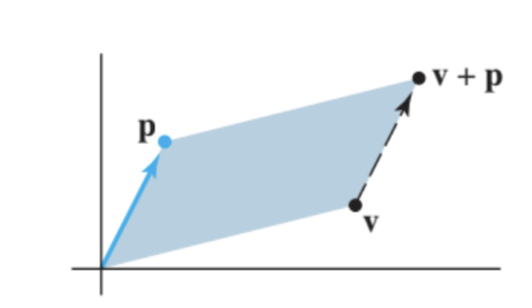
\includegraphics[width=0.3\textwidth]{img/image12.png}}
    \caption{Sumando \textbf{p} a \textbf{v} traslada \textbf{v} a \textbf{v + p}}
  \end{figure}

\begin{tcolorbox}[colback=blue!10!white,colframe=blue!60!black,title=Conjunto solución]
    Suponga que la ecuación $A\mathbf{x} = \mathbf{b}$ es consistente para alguna $\mathbf{b}$ dada y sea $\mathbf{p}$ una solución. El conjunto solución de $A\mathbf{x} = \mathbf{b}$ es el conjunto solución de todos los vectores de la forma $\mathbf{w} = \mathbf{p} + \mathbf{v}_h$, donde $\mathbf{v}_h$ es cualquier solución de la ecuación homogénea $A\mathbf{x}=0$
\end{tcolorbox}

El teorema anterior dice que si $A\mathbf{x} = \mathbf{b}$ tiene una solución, entonces el conjunto solución se obtiene al trasladar el conjunto solución de $A\mathbf{x} = \mathbf{0}$, empleando cualquier solución particular $\mathbf{p}$ de $A\mathbf{x} = \mathbf{b}$ para dicha traslación. Aun cuando $n > 3$, nuestra imagen mental del conjunto solución de un sistema consistente $A\mathbf{x} = \mathbf{b}$ con ($\mathbf{b} \neq 0$) es un solo punto diferente de cero, o una recta o un plano que no pasan por el origen.

\begin{figure}[ht]
    \centerline{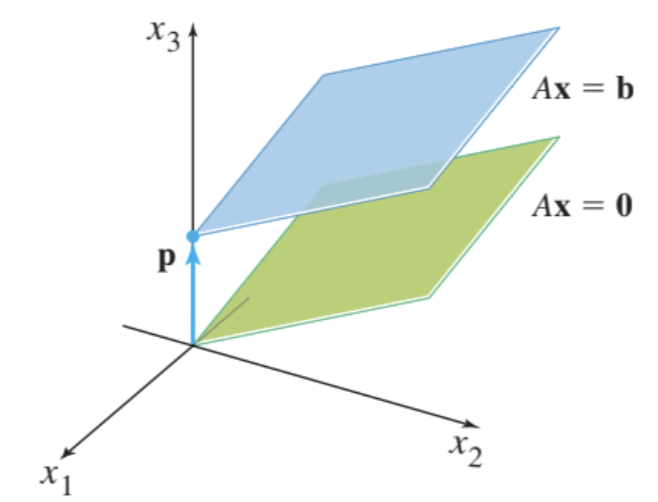
\includegraphics[width=0.3\textwidth]{img/image13.png}}
    \caption{Conjuntos solución paralelos de $A\mathbf{x} = \mathbf{b}$ y $A\mathbf{x} = 0$}
  \end{figure}

Cuando $A\mathbf{x} = \mathbf{b}$ no tiene solución, entonces el conjunto solución es vacío. \cite{DavidC}

\begin{tcolorbox}[colback=green!20!white,colframe=green!80!black,title=Conjunto Solución (de un Sistema Consistente) en Forma Vectorial Paramétrica]
    \begin{itemize}
        \item[1.] Reduzca por filas la matriz aumentada a su forma escalonada reducida
        \item[2.] Exprese cada variable básica en términos de cualquiera de las variables libres presentes en la ecuación.  
        \item[3.] Escriba una solución típica $\mathbf{x}$ como un vector cuyas entradas dependen de las variables libres (si las hay)
        \item[4.] Descomponga $\mathbf{x}$ en una combinación lineal de vectores (con entradas numéricas) empleando las variables libres como parámetros.  
    \end{itemize}
\end{tcolorbox}

\pagebreak

\begin{tcolorbox}[colback=red!10!white, colframe=red!70!black, title=Resumen]
    \begin{itemize}
        \item[-] Un sistema Homogéneo de $m$ ecuaciones con $n$ incógnitas es un sistema lineal de la forma
        \item[] \begin{equation*}
            \begin{matrix}
                \begin{aligned}
                    a_{11}x_1 + a_{12}x_2 + \dots + a_{1n}x_n = 0\\
                    a_{21}x_1 + a_{22}x_2 + \dots + a_{2n}x_n = 0\\
                    \vdots \phantom{aaaaaaaa} \vdots \phantom{aaaaaaaaaa} \vdots \phantom{aaaaaa} \vdots\\
                    a_{m1}x_1 + a_{m2}x_2 + \dots + a_{mn}x_n = 0\\
                \end{aligned}
            \end{matrix}
        \end{equation*}

        \item[-] Un sistema lineal homogéneo siempre tiene la \textbf{solución trivial o solución cero} $$x_1 = x_2 = \dotsb = x_n = 0$$
        \item[-] Las soluciones para un sistema lineal homgéneo diferentes de la trivial se denominan \textbf{soluciones no triviales}
        \item[-] La ecuación homogénea $A\mathbf{x} = 0$ tiene una solución no trivial si y solo si la ecuación tiene al menos una variable libre. 
        \item[-] Un sistema lineal homgéneo tiene al menos una variable libre si ($n > m$)  
        \item[-] Si $A\mathbf{x} = \mathbf{b}$ tiene una solución, entonces el conjunto solución se obtiene al trasladar el conjunto solución de $A\mathbf{x} = \mathbf{0}$, empleando cualquier solución particular $\mathbf{p}$ de $A\mathbf{x} = \mathbf{b}$ para dicha traslación 
    \end{itemize}
\end{tcolorbox}

\bibliography{Referencias}
\end{document}